\documentclass{article}
\usepackage{setspace}
\usepackage{gensymb}
\usepackage{xcolor}
\usepackage{caption}
%\usepackage{subcaption}
%\doublespacing
\singlespacing
\usepackage{float}
%\usepackage{graphicx}
%\usepackage{amssymb}
%\usepackage{relsize}
\usepackage[cmex10]{amsmath}
\usepackage{mathtools}
%\usepackage{amsthm}
%\interdisplaylinepenalty=2500
%\savesymbol{iint}
%\usepackage{txfonts}
%\restoresymbol{TXF}{iint}
%\usepackage{wasysym}
\usepackage{amsthm}
\usepackage{mathrsfs}
\usepackage{txfonts}
\usepackage{stfloats}
\usepackage{cite}
\usepackage{cases}
\usepackage{subfig}
%\usepackage{xtab}
\usepackage{longtable}
\usepackage{multirow}
%\usepackage{algorithm}
%\usepackage{algpseudocode}
\usepackage{enumerate}
\usepackage{mathtools}
%\usepackage{eenrc}
%\usepackage[framemethod=tikz]{mdframed}
	\usepackage{listings}
\usepackage{listings}
    \usepackage[latin1]{inputenc}                                 %%
    \usepackage{color}                                            %%
    \usepackage{array}                                            %%
    \usepackage{longtable}                                        %%
    \usepackage{calc}                                             %%
    \usepackage{multirow}                                         %%
    \usepackage{hhline}                                           %%
    \usepackage{ifthen}                                           %%
  %optionally (for landscape tables embedded in another document): %%
    \usepackage{lscape}     
\usepackage{tikz}
\usepackage{circuitikz}
\usepackage{karnaugh-map}
\usepackage{pgf}
\usepackage{wrapfig}
\usepackage{multicol}
\graphicspath{ {./Images} }
\usepackage{geometry}
\geometry{a4paper,total={200mm,225mm},left=25mm,right=30mm}

\title{\color{cyan}EXERCISE 9.1}

\begin{document}
\maketitle
\vspace{-5truemm}
Write the correct answer in each of the following:
\begin{enumerate}
\item The median of a triangle divides it into two 
\begin{enumerate}
\begin{multicols}{2}
\item triangles of equal area
\item congruent triangles
\item right triangles          
\item isosceles triangles
\end{multicols}
\end{enumerate}
\item In which of the following figures (Fig.9.3), you find two polygons on the same base and between the same parallels?

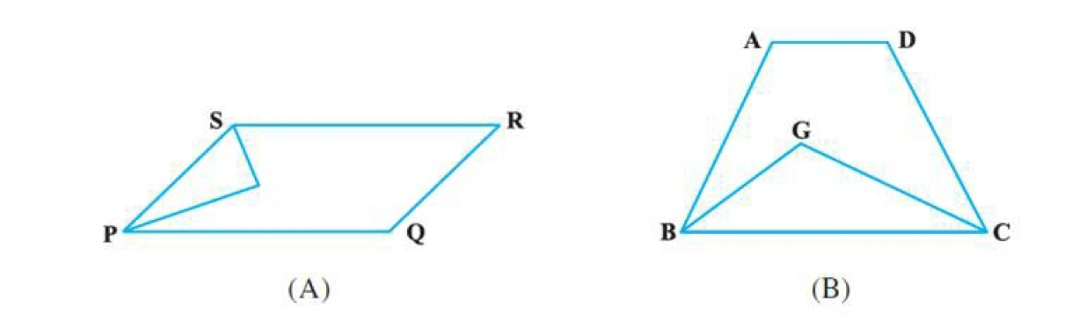
\includegraphics[scale=0.25]{threeone}


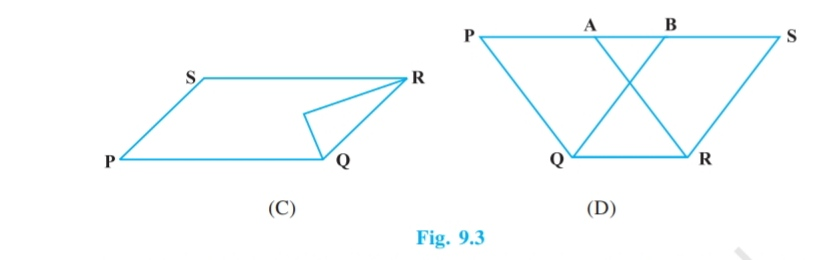
\includegraphics[scale=0.35]{threetwo}

\item The figure obtained by joining the mid-points of the adjacent sides of a rectangle of sides 8cm and 6cm is:
\begin{enumerate}
\begin{multicols}{2}
\item a rectangle of area 24cm$^2$ 
\item a square of area 25cm$^2$
\item a trapezium of area 24cm$^2$ 
\item a rhombus of area 25cm$^2$
\end{multicols}
\end{enumerate}

\item In Fig. 9.4, the area of parallelogram ABCD is:
\begin{enumerate}
\begin{minipage}[b]{0.5\linewidth}
\item AB x BM
\item BC x BN
\item DC x DL
\item AD x DL
\end{minipage}
\begin{minipage}[b]{0.5\linewidth}
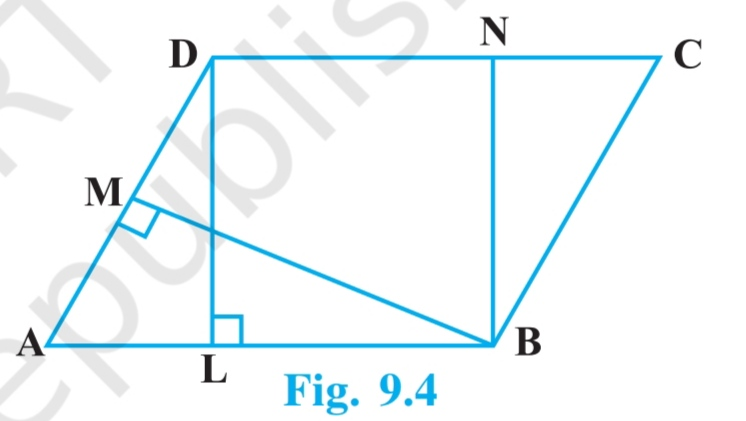
\includegraphics[scale=0.15]{four}
\end{minipage}
\end{enumerate}
\item In Fig. 9.5, if parallelogram ABCD and rectangle ABEF of equal area, then:

\begin{center}
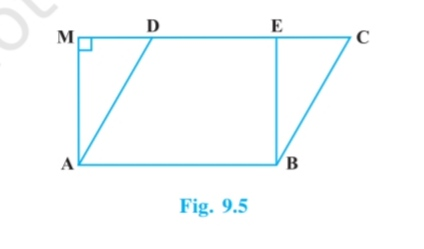
\includegraphics[scale=0.5]{five}
\end{center}
\begin{enumerate}
\item Perimeter of ABCD = Perimeter of ABEM
\item Perimeter of ABCD $<$ Perimeter of ABEM
\item Perimeter of ABCD $>$ Perimeter of ABEM
\item Perimeter of ABCD = 1/2(Perimeter of ABEM)
\end{enumerate}
\item The mid-point of the sides of a triangle along with any of the vertices as the fourth point make a parallelogram of area equal to
\begin{enumerate}
\begin{multicols}{2}
\item 1/2 ar(ABC)  
\item 1/3 ar(ABC)
\item 1/4 ar(ABC)  
\item ar(ABC)
\end{multicols}
\end{enumerate}
\item Two parallelograms are on equal bases and between the same parallels. The ratio of their areas is
\begin{enumerate}
\begin{multicols}{2}
\item 1:2  \item 1:1  \item 2:1  \item 3:1
\end{multicols}
\end{enumerate}
\item ABCD is a quadrilateral whose diagonal AC divides it into two parts, equal in area, then ABCD
\begin{enumerate}
\begin{multicols}{2}
\item is a rectangle       \item is always a rhombus
\item is a parallelogram   \item need not be any of (a), (b) or (c)
\end{multicols}
\end{enumerate}
\item If a triangle and a parallelogram are on the same base an between same parallels, then the ratio of the area of the triangle to the area of the parallelogram is
\begin{enumerate}
\begin{multicols}{2}
\item 1:3  \item 1:2  \item 3:1  \item 1:4
\end{multicols}
\end{enumerate}
\item ABCD is a trapezium with parallel sides AB = a cm and DC = b cm (Fig. 9.6). E and F are the mid-points of the non-parallel sides. The ratio of ar(ABFE) and ar(EFCD) is
\begin{enumerate}
\begin{minipage}[h]{0.65\linewidth}
\item a:b   
\item (3a+b):(a+3b)   
\item (a+3b):(3a+b)
\item (2a+b):(3a+b)
\end{minipage}
\begin{minipage}[h]{0.35\linewidth}
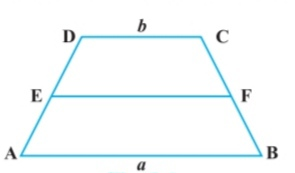
\includegraphics[width=0.75\linewidth]{six}
\end{minipage}
\end{enumerate}
\end{enumerate}

\end{document}

